%!TEX root = informe.tex
\chapter{Objeto}
El objetivo principal de este proyecto es el Análisis de Ciclo de Vida del adoquín común prefabricado del cemento utilizado en obras civiles y urbanismo. Se desea analizar el ciclo de vida del adoquín desde la obtención de la materia prima hasta su fin de vida.

Con este Análisis de Ciclo de Vida se pretende evaluar el comportamiento ambiental de las distintas etapas de su ciclo de vida, las cargas ambientales asociadas a estas etapas e identificar las posibles mejoras.

Para poder conseguir estos objetivos, se pueden establecer los siguientes objetivos básicos:
\begin{itemize}
\item Estudio y análisis de los procesos productivos, de instalación, mantenimiento y reciclado de los adoquines.
\item Análisis de las diferentes metodologías de Análisis de Ciclo de Vida.
\item Elección de una unidad de referencia del producto a partir de la cual se puedan normalizar los datos de entrada y salida y que permita su comparación con otros productos o con etapas de su ciclo de vida del mismo.
\item Desarrollo de un inventario de materiales y procesos de cada etapa del ciclo de vida.
\item Conocer y evaluar los impactos ambientales asociados a cada una de las etapas del producto y a su ciclo completo.
\end{itemize}

A su vez, la redacción del presente proyecto bajo la dirección del Departamento de Expresión Gráfica, Diseño y Proyectos de la Universidad de Málaga tiene como finalidad última la obtención del título de Ingeniero Industrial.

\chapter{Alcance}

En este proyecto se analiza la posibilidad de aprovechar la radiación solar, para la producción de energía eléctrica, en ubicaciones situadas en España y Rumanía, mediante centrales fotovoltaicas conectadas con la red eléctrica.

En el capítulo tres se presenta el consumo de energía eléctrica en el mundo. Para Es- paña se presenta también la evolución de la producción de energía eléctrica en función de su origen y se hace una previsión de la misma para el año 2008. Se hace una presentación de las energías renovables y de su nivel de implantación a nivel mundial, remarcando la energía solar fotovoltaica en España y Rumanía. A continuación, se presentan los principa- les componentes de una central fotovoltaica.

El capítulo cuatro muestra las fuentes de información utilizadas para la realización del proyecto.

En requisitos de diseño (capítulo 6) se presentan las dos ubicaciones inicialmente elegidas para el análisis: Tarragona y Bucarest.

El capitulo siete, análisis de soluciones, presenta los datos de radiación solar y tem- peratura para las dos ubicaciones elegidas inicialmente y también se buscan las ubicaciones con mayor radiación solar en España y Rumanía, presentando también en este caso la ra- diación solar y temperatura. Por último, se hace un análisis económico de las centrales fo- tovoltaicas emplazadas en cada ubicación para determinar el grado de rentabilidad de la inversión en cada caso. Finalmente, el capítulo ocho presenta las mejores soluciones, tanto técnicas como económicas.

\chapter{Antecedentes}

\section{Introducción}\label{sec:introantecedentes}
La mayoría de las ciudades europeas utilizan materiales prefabricados basados en el cemento para urbanizar el terreno transformándolo en espacio público que utilizarán los ciudadanos. Estas instalaciones deben ser resistentes, económicas, funcionales y sobre todo sostenibles. La sostenibilidad es un requisito que ha ido ganando importancia en los últimos años debido no solo al aspecto económico —costes y mantenimiento principalmente— sino también al medioambiental.

El impacto medioambietal que producen las actividades humanas en la naturaleza debería convertirse en un elemento más de estudio en cualquier proyecto de ingeniería actual. Para el caso de este proyecto, el sector de las obras civiles y urbanismo supone un consumo muy elevado de materias primas y energía debido a que representa un porcentaje importante del Producto Interior Bruto de España, lo que implica altas emisiones al medio ambiente \cite{minetur}.

La incorporación de criterios ambientales en la fase de diseño de un producto y/o servicio se denomina \textit{ecodiseño}. El ecodiseño surge como respuesta a la necesidad de introducir estos criterios durante todo el ciclo de vida de un producto con el objetivo de prevenir o reducir su impacto ambiental —principalmente minimizar los residuos, emisiones y costes energéticos \cite{iso14006}. El ecodiseño es el eslabón clave hacia la sostenibilidad y el consumo responsable ya que incorpora nuevos conceptos como la visión de producto-sistema y el ciclo de vida e integra aspectos económicos y sociales como la ecoeficiencia y el ecodiseño sostenible \cite{ihobeeco}.

La metodología del Análisis de Ciclo de Vida (ACV) permite cuantificar todos los procesos relacionados con un producto y/o servicio desde el punto de vista de las \textit{entradas} —materias primas y energía— y \textit{salidas} —emisiones a la tierra, mar o aire y residuos— en el sistema, identificar los puntos clave y establecer una \textbf{estrategia de mejora} \cite{iso14040}.

\begin{figure}[!htb]
\centering
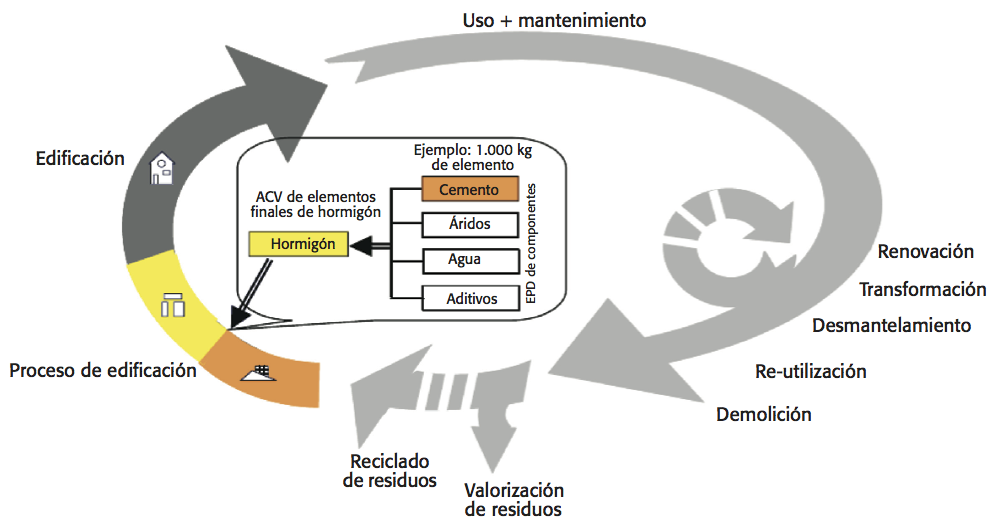
\includegraphics[width=12cm]{ciclodevida.png}
\caption[Ciclo de vida de los prefabricados de cemento.]{Ciclo de vida de los prefabricados de cemento. Fuente: \cite{oficemen}.}
\label{fig:ciclodevidaprefabric}
\end{figure}

\section{Relación entre la construcción y el medioambiente}
El sector de la construcción es uno de los más productivos e importantes tanto social como económicamente. Las infraestructuras construidas aportan calidad de vida al ser humano. Como toda actividad humana, el desarrollo de esta actividad provoca impactos significativos en el medio tanto a la hora de producir, usar y eliminar sus productos \cite{carvalho}.

La concienciación de protección del medio ha obligado al sector a mejorar sus actuaciones en esta materia sin disminuir su capacidad productiva para seguir siendo competitivos. Debe crearse un nuevo paradigma de trabajo en el que el usuario esté satisfecho, el consumo de materia y energía sea mínimo, así como el impacto medioambiental, pero a su vez mejorando la calidad y disminuyendo el tiempo y el coste \cite{augenbroe}.

El impacto medioambiental de un producto cambia según la etapa del ciclo de vida, produciendo diferentes efectos contaminantes sobre el entorno y sobre las personas. Sirva de ejemplos los siguientes datos \cite{carvalho}:
\begin{itemize}
\item el sector de la construcción moviliza un 10\% de la economía mundial y consume un 40\% de la energía mundial producida cada año.
\item según estudios realizados en varios países europeos entre los que se encuentra España, el consumo energético asociado al sector se distribuye en:
  \begin{itemize}
  \item 19\% para la construcción y mantenimiento de edificios.
  \item 48\% para el consumo directo debido a su uso (electricidad, gas, etc.).
  \item 33\% para el transporte.
  \end{itemize}
  \item los residuos de la construcción y demolición (RCD) generados en la Unión Europea superan los 180 millones de toneladas cada año, es decir, 480 kg. por persona y año. Del total de esos residuos, sólo el 28\% son reutilizados \footnote{Como se indica en la sección \ref{sec:ventajas}, en el caso de los adoquines se recupera el 95\%.}.
\end{itemize}

\section{Descripción del ciclo de vida de un producto de la construcción}
Una buena práctica para poder comprende mejor el ciclo de vida de un producto es la estructuración del sistema en procesos, de forma que queden representados todos los subsistemas constituyentes y se pueda identificar claramente un inicio y un final de cada uno.

Un diagrama que represente los flujos de entrada (materiales, energía, productos inacabados) y salida (productos finales, productos inacabados, co-productos, residuos) aporta una visión más clara de las fases del ciclo completo. Con los elementos bien identificados es más fácil atribuirle causas y consecuencias tanto a su subsistema como al sistema completo.

\begin{figure}[!htb]
\centering
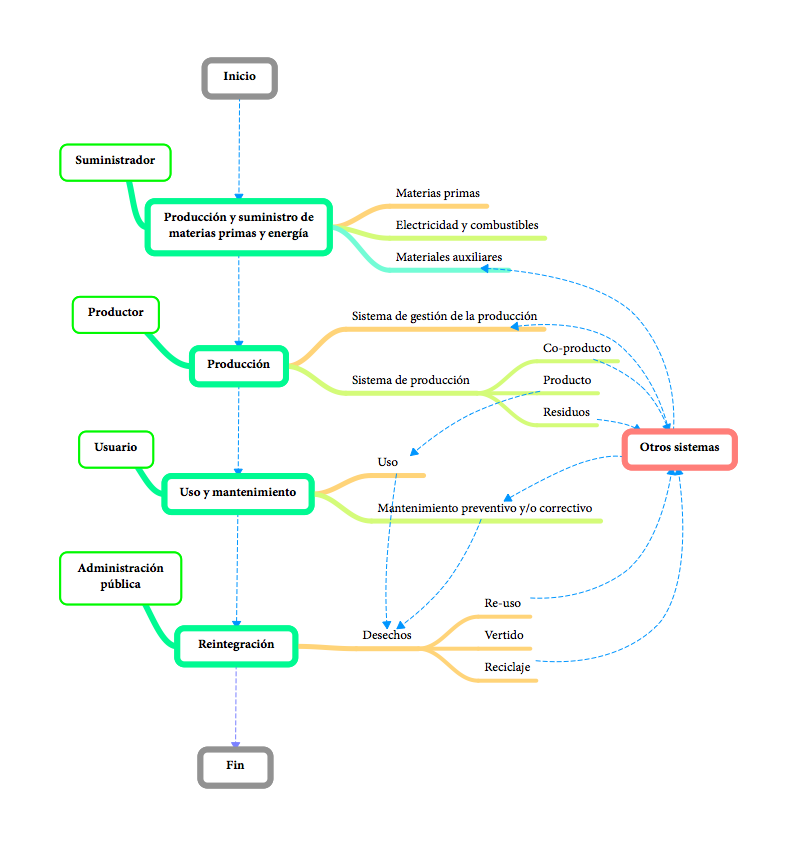
\includegraphics[width=15cm]{flujo_generico_acv.png}
\caption{Flujo genérico del ciclo de vida de un producto.}
\label{fig:flujo_generico_acv}
\end{figure}

El adoquín, se ajusta perfectamente al flujo genérico representado en la figura \ref{fig:flujo_generico_acv}. Las cuatro etapas que se encuentran entre el inicio y el fin serán exactamente los ciclos modelados y analizados en este proyecto.

\section{Impactos potenciales del adoquín al medio ambiente}
A la hora de analizar los aspecto medioambientales de un sistema es necesario establecer diferentes niveles de análisis para poder establecer una estrategia de estudio, ya que a lo largo de la vida de un producto se pueden encontrar diferentes contextos.

\begin{figure}[!htb]
\centering
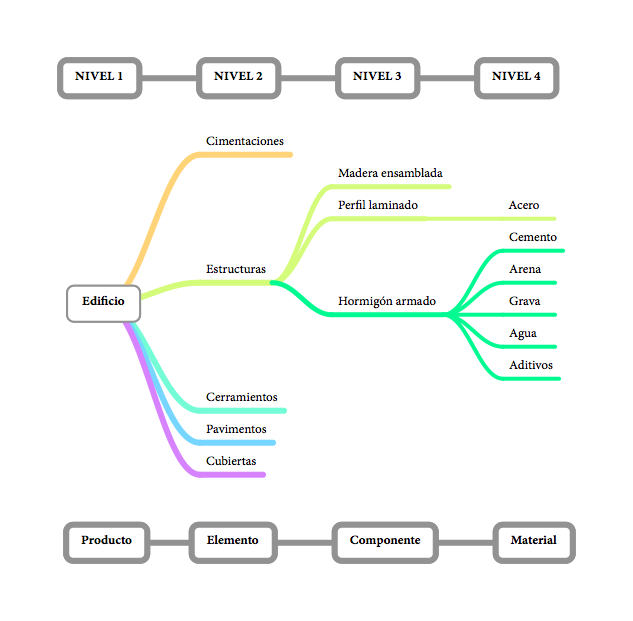
\includegraphics[width=15cm]{niveles_estudio_ciclo_vida.png}
\caption{Niveles de estudio del ciclo de vida.}
\label{fig:niveles_estudio_ciclo_vida}
\end{figure}

Al ser el adoquín un elemento de pavimentación se encontraría en el denominado nivel 2 (ver figura \ref{fig:niveles_estudio_ciclo_vida} ). Los impactos medioambientales del nivel 2 se clasifican según el momento de su vida en:

\begin{itemize}
  \item Producción
    \begin{itemize}
     \item Consumo de energía y recursos naturales en los procesos de producción y transporte.
     \item Producción de ruidos y vibraciones.
     \item Producción de residuos por excedentes de procesos y embalajes.
     \item Emisiones de partículas al aire (p. ej.: polvo).
    \end{itemize}
  \item Uso y mantenimiento
    \begin{itemize}
      \item Consumo de energía y recursos en los procesos de mantenimiento.
      \item Producción de residuos o sustancias tóxicas en función de los procesos de mantenimiento, su naturaleza y vida útil.
    \end{itemize}
  \item Reintegración
    \begin{itemize}
      \item Impactos potenciales traspuestos al producto final que lo utiliza.
    \end{itemize}
\end{itemize}

\section{Prefabricados del cemento. Adoquines}

\subsection{Historia de los adoquines}
A lo largo de la historia de la humanidad se han ido utilizando diferentes tipos de adoquines para pavimentar los suelos urbanos. Los primeros adoquines eran de piedra, obtenidos a partir de los guijarros de río colocados sobre una capa de arena, usando una mezcla de cal y arena como sellante de juntas  \cite{euroadoquin}.

Debido al coste y el ruido del tráfico rodado, en la primera mitad del siglo XIX comenzaron a usarse los adoquines de madera, utilizando para el sellado residuos bituminosos. Su reducida duración y la posterior aparición de los neumáticos hicieron que los adoquines de madera fueran sustituidos por un modelo cerámico, con el que se usaba la misma arena tanto para la base como sellante.

Los adoquines de piedra iniciales seguían siendo más resistentes y además no eran tan deslizantes como los cerámicos. A finales del siglo XIX se fabricó por primera vez el \textbf{adoquín de hormigón}. Estos adoquines proporcionaban una mayor uniformidad que los de piedra, eran muy resistentes y con un coste inferior. Alemania y Holanda fueron los primeros en incorporar este nuevo formato de adoquín a sus núcleos urbanos. Al principio se usaban modelos que imitaban a los de piedra tanto en forma como colocación, pero pronto se añadieron formas dentadas o curvas, permitiendo una mejor alineación con el trazado.

Finalmente, durante la década de los 70 se mejoraron sustancialmente los sistemas de fabricación, permitiendo una gran variedad de modelos de adoquines y un abaratamiento de los costes de fabricación e instalación que llega hasta nuestros días.

\subsection{Ventajas e inconvenientes del uso de adoquines}\label{sec:ventajas}

En comparación con otros tipos de pavimentos tales como los asfálticos o los pavimentos contínuos hormigonados, los adoquines presentan las siguientes ventajas:

\begin{itemize}
\item Fabricación: no se utilizan derivados del petróleo, que suelen ser caros y contaminantes, además de requerir una mayor aportación de energía durante el proceso de fabricación. En contraposición, pueden utilizarse cementos y áridos locales, disminuyendo los costes de transporte.

El proceso de fabricación de los adoquines requiere una maquinaria específica debido a que son sometidos a presión y vibración para segurar una resistencia y durabilidad adecuadas. Esto implica un control sobre la fabricación, consistencia y fiabilidad del producto mayor que el resto de pavimentos.

\item Instalación: aunque los adoquines pueden colocarse de forma automatizada, están diseñados de base para ser colocados manualmente, permitiendo instalarse en zonas de difícil acceso, cargas elevadas (muelles de carga, aeropuertos, \ldots), resolver trazados complejos o pendientes pronunciadas. A diferencia de los pavimentos asfálticos, su ejecución no depende de la temperatura ambiente y pueden ser utilizados inmediatamente después de su finalización, lo que implica una reducción en los tiempos de ejecución de obra.

\item Comportamiento: los adoquines pueden ser diseñados para ser muy resistentes tanto a cargas verticales (distribuidas o puntuales) como a esfuerzos horizontales (aceleración-frenada, giros,\ldots). Además, soportan bien sin degradarse los vertidos de aceites y combustibles sobre el pavimento. Los niveles de ruido generados por el tráfico son similares o inferiores a otros pavimentos en ausencia de humedad y sensiblemente inferiores en condiciones de humedad, especialmente a bajas velocidades. La resistencia a deslizamiento es mayor al del resto de pavimentos.

\item Mantenimiento: la vida útil del adoquín viene determinada principalmente por el comportamiento de la base, subbase y explanada y no por el propio adoquín. La vida útil \footnote{La vida útil se considera como la duración estimada que un objeto puede tener cumpliendo correctamente con la funcion para la cual ha sido creado.} de cálculo suele ser a 30 años, aunque en condiciones normales puede superar los 50 años. De esta manera, al renovar el pavimento se puede reutilizar un 95\% de los adoquines originales \cite{euroadoquin}. El adoquín es la mejor opción en zonas donde aún no se han implantado todos los servicios de públicos debido a que pueden ser levantados fácilmente para llevar tareas de instalación o reparación en el subsuelo. La conservación de los adoquines se limita al relleno de juntas erosionadas con arena de sellado cada cierto tiempo y a la reposición de adoquines fracturados.

\item Costes: aunque inicialmente el precio del metro cuadrado instalado es algo superior a otros pavimentos, a largo plazo es mucho más barato debido al menor mantenimiento y la reutilización de piezas. Los pavimentos asfálticos y hormigonados requieren un mayor esfuerzo e inversión a la hora de ser reparados o retirados para acceder al subsuelo \cite{pavimentos,euroadoquin}.

\item Aspecto estético: actualmente los adoquines pueden diseñarse de todas formas, texturas, colores y disposiciones según las necesidades de la obra.
\end{itemize}


Realmente el uso de adoquines apenas tiene inconvenientes, aunque existen varios, entre los que destacan:

\begin{itemize}
  \item Incomodidad: debido a que el pavimento está lleno de juntas de separación entre adoquines y poco a poco se vuelve irregular, la circulación y el paso pueden ser incómodos y conllevar mayores costes de operación a los vehículos.
  \item Nieve: el pavimento de adoquines suele ser irregular y no permite bien la retirada de nieve en zonas con climas donde nieva mucho. Por otro lado, la nieve se derrite antes en pavimentos de asfalto, de color negro, debido al calentamiento del sol.
\end{itemize}

\section{Materias primas de los prefabricados del cemento}
Las características de las materias primas que se pueden emplear en la fabricación de los adoquines se contemplan en la norma UNE EN 1338:2004/AC:2006. En ella se especifican detalladamente los materiaes, propiedades, requisitos y métodos de ensayo de los adoquines prefabricados de hormigón no armados y accesorios complementarios, previstos para uso peatonal, uso en áreas sometidas a tráfico de vehículos y cubiertas, como por ejemplo: aceras, límites de áreas, sendas para bicicletas, aparcamientos, carreteras, autopistas, áreas industriales, aeropuertos, estaciones de autobuses y gasolineras. Esta norma no trata la visibilidad y la tactibilidad de los adoquines ni los adoquines permeables.

\subsection{Cemento}
El cemento es un conglomerante, formado a partir de arcilla y caliza (\ce{CaCO3}), que se endure al mezclarse con agua. Para producir cemento (ver figura \ref{fig:cemento}), la arcilla y la caliza se muelen juntas. A esta mezcla se le añade yeso para conferirle la propiedad de fraguar y endurecerse. El resultado se introduce en un horno rotatorio, normalmente seco por ser más eficiente energéticamente, a una temperatura aproximada de 1450\si{\celsius}. A continuación se introduce el material en un incinerador donde el calentamiento produce la liberación del \ce{CO2} de la caliza y se produce el cemento \emph{clinker}.

\begin{center}
\ce{CaCO3 + calor -> CaO + CO2}
\end{center}

El clinker es el óxido de calcio (\ce{CaO}) obtenido de la reacción anterior, que puede encontrarse acompañado de otros minerales como hierro, aluminio o silicio. El aporte de calor necesario para obtener el clinker representa la mayor parte del coste energético en la producción de cemento.

Por último, se produce la molienda del clinker junto yeso y otros materiales (bauxita, arena,\ldots) para mejorar sus propiedades, produciendo el cemento.

\begin{figure}[!htb]
\centering
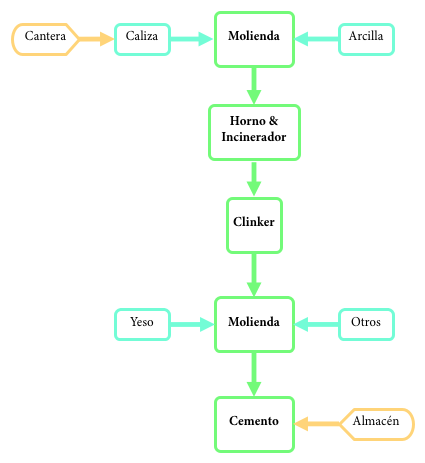
\includegraphics[width=12cm]{cemento.png}
\caption{Diagrama de flujo de la fabricación del cemento.}
\label{fig:cemento}
\end{figure}

Cuando se utiliza la palabra \emph{cemento} se refiere normalmente a un cemento tipo Portland (supone un 95\% de la producción de cementos \cite{jsjunnesson}), nombre no comercial que implica un proceso de producción y una composición característicos. De acuerdo a la norma UNE-EN 197-1:2011 \cite{une1971}, el cemento se divide en tres grupos en función de la cantidad de cemento Portland incluido: CEM I, CEM II y CEM III. El CEM I (95\% a 100\% de contenido de cemento Portland) es el más usado en la fabricación de adoquines.

Con respecto a la normativa específica de adoquines, la norma UNE 80301:1996 \cite{une80301} en el ámbito de España establece los requisitos que debe tener el cemento común. Si se utilizan cementos especiales se recurrirá a la norma UNE 80303:2013, y si son blancos a la norma UNE 80305:2012.

\subsection{Áridos}
Los áridos (entre los que se incluye la arena) son particulas de roca puede ser tanto gravas (piedras de forma natural) como macadán (piedras trituradas), teniendo cada tipo una textura diferente (figura \ref{fig:aridosnaturalesytriturados}). Se pueden añadir diferentes tamaños de áridos para ejercer una función diferente según el mismo. Fracciones menores rellenarán las cavidades que haya entre partículas mayores, aportando adherencia a costa de un mayor peso.

\begin{figure}[!htb]
\centering
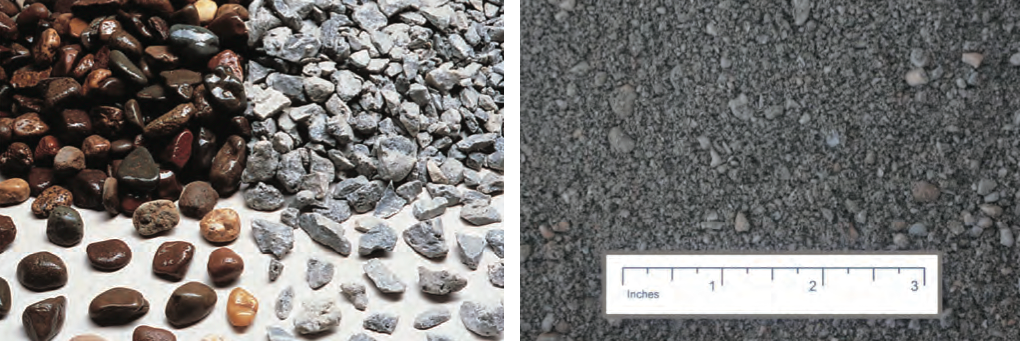
\includegraphics[width=13cm]{aridos.png}
\caption[Áridos naturales y triturados. Granulometrías.]{Áridos naturales y triturados. Granulometrías. Fuente: \cite{sustpave}.}
\label{fig:aridosnaturalesytriturados}
\end{figure}

El material de machaqueo para la producción de macadán se criba para eliminar las partículas menores. Debido a que las partículas que forman el macadán son más irregulares, es más fiable como material de relleno por su capacidad de incrustamiento (la grava tiene una forma más redondeada). El macadán se puede ser utilizado de forma más generalizada en función de la localización ya que la grava natural es un recurso más limitado.

La fuente de recursos de áridos son principalmente de río, mina o cantera o piedras trituradas (macadán). La granulometría de los áridos que se utilicen deberá cumplir las características indicada en la norma UNE EN 1338:2004/AC:2006.

\subsection{Agua}
El agua es muy importante en la constitución del hormigón. Reacciona químicamente con el cemento —hidratación— para proporcionar las propiedades deseadas del hormigón \cite{nrmca}. El agua de amasado es la cantidad de agua que toma contacto con el cemento y se usa para determinar las proporciones del resto de elementos para formar la mezcla. La fuerza y la durabilidad del cemento viene dado en gran parte por la cantidad de agua.

Además de su cantidad, la calidad del agua utilizada tiene efectos importantes en las propiedades del hormigón fresco, tales como el tiempo de fraguado y la facilidad de trabajo. También tiene importantes en la fuerza y durabilidad del hormigón endurecido.

\subsubsection{Fuentes posibles de agua}

Por norma general el agua adecuada para el consumo humano —agua potable— es válida. No obstante, el agua no potable puede ser utilizada siempre que no tenga un impacto negativo en las propiedades del hormigón. La mayoría de las plantas tienen una fuente de agua municipal que proporciona potable sin pruebas de calidad. En zonas rurales o en plantas portátiles in situ —instaladas y desinstaladas en el propio lugar del proyecto—, habrá que utilizar fuentes de agua no potable como ríos o masas de agua.

Otra fuente de agua es la reciclada de la limpieza —agua de lavado— de la mezcladora y otros elementos de la planta. También se podrá aprovechar el agua de precipitaciones atmosféricas que pueda recolectarse en las instalaciones de la planta.

El agua de procesado no sólo se genera de la fabricación del hormigón, sino también del lavado del hormigón reciclado. Los sistemas de recolección procesan el agua con el cemento y los áridos en forma de lechada que puede ser también utilizada como agua para la mezcla de hormigón.

Las normativas medioambientales suelen requerir que las plantas de fabricación traten y procesen tanto el agua de lluvia como el de procesado —agua de operaciones— para que adquiera ciertos niveles de pH y contenidos sólidos antes de que abandonen las instalaciones \cite{ermco}.

\subsubsection{Cualificación del agua no potable}
El agua es el recurso más importante para el ser humano. En algunas zonas el suministro de agua potable es muy escaso. El uso de fuentes de agua no potables para la producción de hormigón mantiene una producción sostenible de hormigón conservando los recursos de agua potable. La gestión del agua procedente de la producción de hormigón conforme con las normativas medioambientales representa un coste adicional para el fabricante, por lo que el uso de agua no potable representa un ahorro considerable en la producción de hormigón. Cuando se utilizan fuentes de agua no potable es importante verificar y documentar que las impurezas que contiene no merman las características del hormigón, ya que las fuentes pueden contener aceites, grasas, sales disueltas y otros elementos no controlados. Por esta razón, el fabricante debería tener en cuenta que su uso implica un coste adicional que evaluar y controlar.

\subsection{Aditivos}
Se podrán utilizar adiciones o aditivos siempre que produzcan el efecto deseado (acelerante, retardante,\ldots) y no afecte a las características esperadas del hormigón.

\section{Origen del estudio}
Malaka de Prefabricados es una empresa malagueña que inició su actividad en 1994. Su compromiso consistía en integrarse en el tejido industrial de la provincia, estableciendo lazos con otras industrias locales, y apostar por un producto de calidad que marcara la diferencia en el mercado sin repercutir en el precio.

\begin{figure}[!htb]
\centering
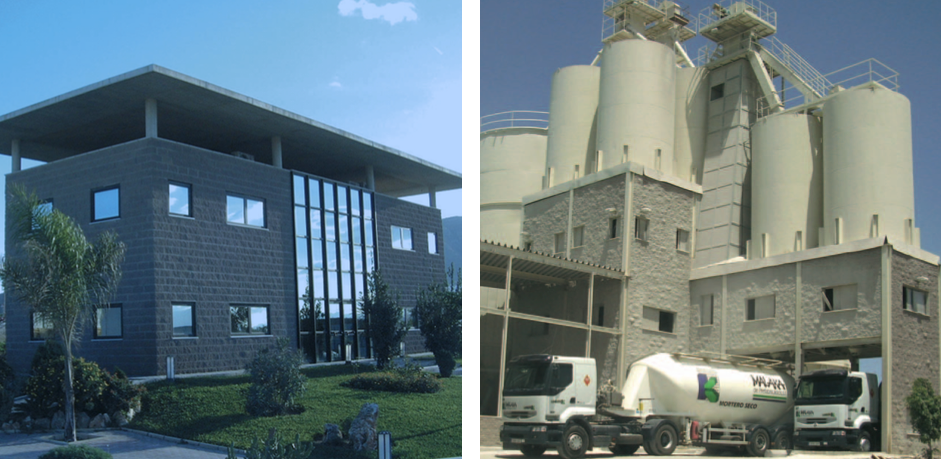
\includegraphics[width=15cm]{malaka1.png}
\caption[Instalaciones de Malaka de Prefabricados.]{Instalaciones de Malaka de Prefabricados. Fuente: \protect\cite{malakacatalogo}.}
\label{fig:malakainstalaciones1}
\end{figure}

A finales de la década de los 90 y principios del nuevo milenio experimentaron un fuerte crecimiento como consecuencia del rápido auge del sector de la construcción en Andalucía, convirtiéndose en un referente de los prefabricados en la provincia y en la comunidad autónoma.

Sus principales líneas de producción son los adoquines, bloques y bordillos de hormigón, a los que se dedica por completo una planta de producción automatizada. La línea de adoquines dispone de varias gamas de producto debido a la versatilidad y demanda de la que disfruta. El resto de productos —tubos, registros, aligerantes, casetones y mortero seco ensilado— se fabrican en la segunda planta.

\begin{figure}[!htb]
\centering
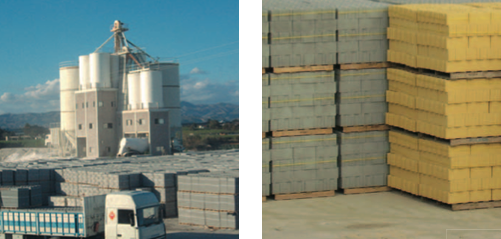
\includegraphics[width=15cm]{malaka2.png}
\caption[Instalaciones accesorias de Malaka de Prefabricados.]{Instalaciones accesorias de Malaka de Prefabricados. Fuente: \protect\cite{malakacatalogo}.}
\label{fig:malakainstalaciones2}
\end{figure}

El compromiso de calidad en sus productos pasó por cumplir todos los requisitos de la normativa española y europea, adoptando el marcado CE como sello de calidad. Tanto clientes como partners pueden dar muestra de su confianza en la calidad de los mismos. Entre sus principales proyectos se encuentran el Palacio de Deportes Martín Carpena (Ferrovial—Agroman), el Parque Temático de Melilla (Dragados) y colaboraciones con los ayuntamientos de Marbella y Estepona.

Durante los casi veinte años en la industria han intentado adoptar las mejores y más novedosas tecnologías de fabricación del sector, ampliando de forma progresiva el tamaño de sus instalaciones en la Finca Pizarro, a las afueras de la ciudad de Málaga.

La empresa adoptó a principios de 2000 la Certificación de Sistemas de Gestión de la Calidad (ISO 9001) y varios años más tarde la Certificación Sistemas de Gestión Ambiental (ISO 14000) como referente de compromiso con la calidad de su producción y con el medioambiente.

\section{Metodología}

XXXX EXPLICAR MEJOR UNA VEZ TERMINADO EL PROYECTO XXXX
El presente proyecto seguirá el siguiente proceso de estudio:

\begin{itemize}
  \item En primer lugar se establecen las características del producto a estudio, historia de su desarrollo y materias primas que lo componen.
  \item Se expondrá la relevancia del producto con el impacto medioambiental y se explicará la metodología de Análisis de Ciclo de Vida, su importancia y las herramientas con las que se trabajará.
  \item A continuación se realizará un Análisis de Ciclo de Vida del producto desde ``la cuna hasta la tumba'', es decir: extracción de materias primas, fabricación, instalación, uso y mantenimiento, y fin de vida.
  \item Una vez analizados, se hará una comparación entre ellos.
  \item Por último, se desarrollarán las conclusiones obtenidas del estudio y posibles mejoras o futuras líneas de expansión.
\end{itemize}

\chapter{Normas y referencias}
\section{Disposiciones legales y normas aplicadas}

Para la realización de este proyecto se han tenido en cuenta la siguiente normativa:

\begin{itemize}
  \item UNE-EN-ISO 14040:2006, Gestión Ambiental. Análisis de ciclo de vida. Principios y marco de referencia.
  \item UNE-EN-ISO 14440:2006, Gestion Ambiental. Análisis de ciclo de vida. Requisitos y directrices.
  \item UNE-EN-ISO 150041EX:1998, Análisis de ciclo de vida simplificado.
  \item UNE-EN-ISO 14006:2011, Sistemas de gestión ambiental. Directrices para la incorporación del ecodiseño.
  \item UNE-EN 1338:2004/AC:2006 Adoquines de hormigón. Especificaciones y métodos de ensayo.
  \item UNE-EN 197-1:2011 La norma europea de especificaciones de cementos comunes.
  \item UNE 80301:1996 Cementos. Cementos comunes. Composicion, especificaciones y criterios de conformidad.
  \item UNE 127338:2007 Propiedades y condiciones de suministro y recepción de los adoquines de hormigón. Complemento nacional a la Norma UNE EN 1338.
  \item UNE-CEN/TR 15941:2011 IN Sostenibilidad en la construcción. Declaraciones ambientales de producto. Metodología para la selección y uso de datos genéricos.
  \item UNE-EN15804:2012 Sostenibilidad en la construcción.Declaracionesambientales de producto.
  \item UNE-EN 15978:2012 Sostenibilidad en la construcción. Evaluación del comportamiento ambiental de los edificios. Métodos de cálculo.
  \item ISO. UNE-ISO 21930 Sostenibilidad en la construcción de edificios. Declaración ambiental de productos de construcción.
\end{itemize}

\bibliographystyle{plain}
\bibliography{informe}

\section{Programas de cálculo}

El software de Análisis de Ciclo de Vida elegido es SimaPro de PRé Consultants.

Los cálculos se han realizado mediante la aplicación de hoja de cálculo Apple Numbers.app.

\section{Plan de gestión de la calidad aplicado durante la redacción del Proyecto}

Para la realización de este proyecto se ha aplicado la siguiente normativa:
\begin{itemize}
  \item UNE 157001:2002 Criterios generales para la elaboración de proyectos.
  \item UNE 50132:1994 Documentación. Numeración de las divisiones y subdivisiones en los documentos escritos.
  \item UNE 1027:1995 Dibujos técnicos. Plegado de planos.
  \item UNE 1032:1982 Dibujos técnicos. Principios generales de representación.
  \item UNE 1035:1995 Dibujos técnicos. Cuadro de rotulación.
  \item UNE 1039:1994 Dibujos técnicos. Acotación. Principios generales, definiciones, métodos de ejecución e indicaciones especiales.
\end{itemize}

Durante la redacción de este proyecto se han corroborado los datos aportados por el fabricante. Se han revisado errores de transcripción de datos, fallos en los cálculos, así como errores gramaticales y ortográficos. Además, se ha comprobado la consistencia de los conceptos de estudio con la metodología empleada. Por último, se ha utilizado un sistema de copia de seguridad basada en control de versiones, por la cual los datos pueden ser recuperados o consultados en cualquier momento.

\chapter{Definiciones y abreviaturas}
\begin{itemize}
  \item AENOR (Asociación Española de Normalización y Certificación): entidad de certificación de sistemas de gestión, productos y servicios, y responsable del desarrollo y difusión de las normas UNE.
  \item Análisis del Ciclo de Vida (ACV): recopilación y evaluación de las entradas, las salidas y los impactos ambientales potenciales de un sistema del producto a través de su ciclo de vida.
  \item Análisis del Inventario del Ciclo de Vida (ICV): fase del análisis del ciclo de vida que implica la recopilación y la cuantificación de entradas y salidas para un sistema del producto a través de su ciclo de vida.
  \item Aspecto ambiental: elemento de las actividades, productos o servicios de una organización que puede interactuar con el medio ambiente.
  \item BUWAL: Bundesamt für Unwelt, Wald und Landshaft. Oficina Federal de Medio Ambiente, Bosque y Campo (Suiza).
  \item Categoría de impacto: clase que representa asuntos ambientales de interés a la cual se pueden asignar los resultados del análisis del inventario del ciclo de vida.
  \item CEN: Comité Europeo de Normalización.
  \item Ciclo de vida: etapas consecutivas e interrelacionadas de un sistema del producto, desde la adquisición de materia prima o de su generación a partir de recursos naturales hasta la disposición final.
  \item De la cuna a la tumba: expresión que referencia al ciclo de vida de un producto desde la extracción de las materias primas hasta la disposición.
  \item Eco-Indicador: indicador ambiental, desarrollado por PRé Consultants para el gobierno de Holanda.
  \item Ecodiseño: diseño que considera acciones orientadas a la mejora ambiental del producto o servicio en todas las etapas de su ciclo de vida, desde su creación en la etapa conceptual, hasta su tratamiento como residuo.
  \item Emisiones atmosféricas: introducción en la atmósfera por el hombre, de forma directa o indirecta, de sustancias o energía que tengan una acción perjudicial para la salud humana o el medio ambiente.
  \item Evaluación del Impacto del Ciclo de Vida (EICV): fase del análisis del ciclo de vida en la que los hallazgos del análisis del inventario o de la evaluación del impacto, o de ambos, se evalúan en relación con el objetivo.
  \item Impacto ambiental: alteración apreciable sobre la salud y bienestar de cualquier ser vivo o sobre el medio ambiente. En relación al ACV, se trata de la anticipación razonable a un efecto.
  \item ISO (International Standard Organitation). Organización Internacional de Estándares.
  \item Life Cycle Assessment (LCA): acrónimo en inglés de Análisis de Ciclo de Vida.
  \item Límite del sistema: conjunto de criterios que especifican cuales de los procesos unitarios son parte de un sistema del producto.
  \item Medio ambiente: conjunto de factores físico-químicos (agua, aire, clima, etc.), biológicos (fauna, flora y suelo) y socioculturales (asentamiento y actividad humana, uso y disfrute del territorio, formas de vida, etc.) que integran el entorno en que se desarrolla la vida del hombre y la sociedad (RD 4/1986 de 23 de enero 1986).
  \item Proceso unitario: elemento más pequeño considerado en el análisis del inventario del ciclo de vida para el cual se cuantifican datos de entrada y salida.
  \item Producto evitado: aquel material o producto que no es necesario generar debido a que ya se ha obtenido durante los procesos de otro producto.
  \item UNE: Una Norma Española.
  \item UNE-EN: Una Norma Española que además es Norma Europea (European Norm) a través del CEN.
  \item UNE-EN-ISO: Adaptación de normativa ISO a ámbito europeo por el CEN y de ahí al ámbito español por AENOR.
  \item Unidad funcional: aquella prestación o función que realiza un producto que permite su comparación con otros.
  \item Vida útil: duración estimada que un objeto puede tener cumpliendo correctamente con la función para la cual ha sido creado.
\end{itemize}
